\documentclass[dvipsnames,11pt]{article}
\usepackage{amsmath}

%Hey, if you're using this preamble it means that it was probably written by Stefano Graziosi (me). If you see something that doesn't make sense, feel free to email me at stefano.graziosi@studbocconi.it
%p.s. in case it's not already evident from the preamble, I'm not a professional LaTeX user, so I'm sure there are better ways to do things. I'm just trying to make it work.

%------------------------------------------------------------------------------
%           LAST UPDATE: 30-01-2025
%------------------------------------------------------------------------------

%I don't own copyright on anything, I just literally copied and pasted together a bunch of stuff.

%Credit goes to the original authors.

%------------------------------------------------------------------------------
%           Packages
%------------------------------------------------------------------------------

\usepackage{fancyhdr}
\usepackage[dvipsnames]{xcolor}
\usepackage[many]{tcolorbox}
\usepackage[all]{xy}
\usepackage{tcolorbox}
\usepackage{graphicx}
\usepackage{hyperref}
\usepackage{xcolor}    
\usepackage{wrapfig}
\usepackage{amsmath, amssymb, amsthm}
\usepackage{titlesec}
\usepackage{halloweenmath}
\usepackage{enumitem}
\usepackage{listings}
\usepackage{kantlipsum}
\usepackage{pdfpages}

\usepackage[T1]{fontenc}                            % Font Styling
\usepackage{lmodern,mathrsfs}


\usepackage{mathtools,amsthm,amssymb,amsfonts,bm}   % Math Presets
\usepackage{thmtools,amsmath}
\usepackage{array,tabularx,booktabs}                % Table Presets
\usepackage{graphicx,wrapfig,float,caption}         % Figure Presets
\usepackage{setspace,multicol}                      % Text Presets
\usepackage{tikz,physics}                           % Physics Presets

\usepackage{titlepic}
\usepackage{pdfpages}

%------------------------------------------------------------------------------
%           Geometry
%------------------------------------------------------------------------------

\usepackage[a4paper,margin=1in]{geometry}
%\usepackage[margin=1in]{geometry}

%------------------------------------------------------------------------------
%           Chapter and section formatting
%------------------------------------------------------------------------------

%\renewcommand{\chaptername}{Lecture}
%\renewcommand\thesection{P~\arabic{section}}

\renewcommand{\thefigure}{\thesection-\arabic{figure}}
\renewcommand{\thetable}{\thesection-\arabic{table}}

%------------------------------------------------------------------------------
%           Colours
%------------------------------------------------------------------------------

\definecolor{sgblue}{rgb}{0, 169, 211}
\definecolor{sggreen}{rgb}{0, 164, 0}
\definecolor{sgpurple}{rgb}{99, 0, 165}
\definecolor{sgyellow}{rgb}{255, 211, 0}
\definecolor{sgorange}{rgb}{255, 127, 20}

\definecolor{sbblue}{rgb}{219, 248, 254}
\definecolor{sbgreen}{rgb}{223, 255, 218}
\definecolor{sbpurple}{rgb}{241, 220, 255}

\definecolor{codegreen}{rgb}{0,0.6,0}
\definecolor{codegray}{rgb}{0.5,0.5,0.5}
\definecolor{codepurple}{rgb}{0.58,0,0.82}
\definecolor{backcolour}{rgb}{0.95,0.95,0.92}

%------------------------------------------------------------------------------
%           Environments
%------------------------------------------------------------------------------

%Standard \latex box

\newtcolorbox{mybox}[3][]
{
  colframe = #2!25,
  colback  = #2!10,
  coltitle = #2!20!black,  
  title    = {#3},
  #1,
}

%Standard "Problem" environment

\newtheorem{problem}{Problem}

%Personalised "Solution" environment

\newenvironment{solution}[1][\it{\textcolor{MidnightBlue}{Solution}}]{\textbf{#1. } }{\textcolor{MidnightBlue}{$\square$}}


% ----------------------------------------------------------------------
%           Special Environments 
% ----------------------------------------------------------------------

\newlength{\spacelength}
\settowidth{\spacelength}{\normalfont\ }
\declaretheoremstyle[
    headfont={\bfseries\sffamily\footnotesize},
    notefont={\normalfont},
    bodyfont={\normalfont},
    headpunct={\relax},%\newline,
    headformat={%
        \makebox[0pt][r]{\NAME\ \NUMBER\hspace{\marginparsep}}\hskip-\spacelength{\normalsize\NOTE}},
]{theorem}

\tcolorboxenvironment{theorem}{
  boxrule=0pt,
  boxsep=0pt,
  colback={White},
  enhanced jigsaw, 
  borderline west={1pt}{0pt}{ForestGreen},
  sharp corners,
  before skip=10pt,
  after skip=10pt,
  left=5pt,
  right=5pt,
  breakable,
}

\declaretheorem[style=theorem]{proposition}

\let\proof\relax
\let\endproof\relax

\declaretheoremstyle[
    headfont={\bfseries\sffamily\footnotesize},
    notefont={\normalfont},
    bodyfont={\normalfont},
    headpunct={\relax},%\newline,
    headformat={%
        \makebox[0pt][r]{\NAME\ \NUMBER\hspace{\marginparsep}}\hskip-\spacelength{\normalsize\NOTE}},
]{theorem}

\tcolorboxenvironment{proposition}{
  boxrule=0pt,
  boxsep=0pt,
  colback={White},
  enhanced jigsaw, 
  borderline west={1pt}{0pt}{Mulberry},
  sharp corners,
  before skip=10pt,
  after skip=10pt,
  left=5pt,
  right=5pt,
  breakable,
}

\declaretheorem[style=theorem]{theorem}

\let\proof\relax
\let\endproof\relax

\declaretheoremstyle[
    headfont={\small\scshape},
    notefont={\normalfont},
    bodyfont={\normalfont},
    headpunct={\relax},
    headformat={%
        \makebox[0pt][r]{\NAME\hspace{\marginparsep}}\hskip-\spacelength{\NOTE}},
]{proof}

\tcolorboxenvironment{proof}{
  boxrule=0pt,
  boxsep=0pt,
  blanker,
  borderline west={1pt}{0pt}{black},
  before skip=10pt,
  after skip=10pt,
  left=5pt,
  right=5pt,
  breakable,
}

\declaretheoremstyle[
    headfont={\footnotesize\itshape},
    notefont={\normalfont},
    bodyfont={\normalfont},
    headpunct={\relax},
    headformat={%
        \makebox[0pt][r]{\NAME\hspace{\marginparsep}}\hskip-\spacelength{\NOTE}},
]{claim}

\declaretheorem[
    style=proof,
    qed=\qedsymbol]{proof}

\declaretheorem[style=claim]{Intuition}

\theoremstyle{theorem}
\newtheorem{ques}{Question}

\theoremstyle{theorem}
\newtheorem{definition}{Definition}
\tcolorboxenvironment{definition}{
  boxrule=0pt,
  boxsep=0pt,
  colback={White},
  enhanced jigsaw, 
  borderline west={1pt}{0pt}{Cerulean},
  sharp corners,
  before skip=10pt,
  after skip=10pt,
  left=5pt,
  right=5pt,
  breakable,
}

\theoremstyle{theorem}
\newtheorem{lemma}{Lemma}
\tcolorboxenvironment{lemma}{
  boxrule=0pt,
  boxsep=0pt,
  blanker,
  borderline west={1pt}{0pt}{Rhodamine},
  before skip=10pt,
  after skip=10pt,
  sharp corners,
  left=5pt,
  right=5pt,
  breakable,
}

\theoremstyle{theorem}
\newtheorem{remark}{Remark}
\tcolorboxenvironment{remark}{
  boxrule=0pt,
  boxsep=0pt,
  colback={White},
  enhanced jigsaw, 
  borderline west={1pt}{0pt}{BurntOrange},
  before skip=10pt,
  after skip=10pt,
  sharp corners,
  left=5pt,
  right=5pt,
  breakable,
}

\theoremstyle{theorem}
\newtheorem{corollary}{Corollary}
\tcolorboxenvironment{corollary}{
  boxrule=0pt,
  boxsep=0pt,
%  colback={White!100!WildStrawberry},
  enhanced jigsaw,
  borderline west={1pt}{0pt}{WildStrawberry},
  before skip=10pt,
  after skip=10pt,
  sharp corners,
  left=5pt,
  right=5pt,
  breakable,
}

\theoremstyle{theorem}
\newtheorem{example}{Example}
\tcolorboxenvironment{example}{
  boxrule=0pt,
  boxsep=0pt,
  blanker,
  borderline west={1pt}{0pt}{Dandelion},
  before skip=10pt,
  after skip=10pt,
  sharp corners,
  left=5pt,
  right=5pt,
  breakable,
}


\theoremstyle{claim}
\newtheorem{intu}{Intuition}

\theoremstyle{claim}
\newtheorem{solu}{Solution}

%------------------------------------------------------------------------------
%           Code Listing Environment
%------------------------------------------------------------------------------

\lstdefinestyle{mystyle}{
    backgroundcolor=\color{backcolour},   
    commentstyle=\color{codegreen},
    keywordstyle=\color{magenta},
    numberstyle=\tiny\color{codegray},
    stringstyle=\color{codepurple},
    basicstyle=\ttfamily\footnotesize,
    breakatwhitespace=false,         
    breaklines=true,                 
    captionpos=b,                    
    keepspaces=true,                 
    numbers=left,                    
    numbersep=5pt,                  
    showspaces=false,                
    showstringspaces=false,
    showtabs=false,                  
    tabsize=2
}

\lstset{style=mystyle}

\setlength{\headheight}{25pt} % Non so perché ma senza questo da un piccolo errore

\pagestyle{fancy}
\fancyhf{} 
\fancyhead[L]{\textsc{\footnotesize{PhD in Economics and Finance} \\ \small{40313 Introd. to Probability}}} 
\fancyhead[R]{\textsc{\small Graziosi \\ Natalucci}} 
\fancyhead[C]{\textbf{Problem set 2}}
\fancyfoot[C]{\thepage} 
\renewcommand{\headrulewidth}{0.4pt} 
\renewcommand{\footrulewidth}{0pt}

\begin{document}

\section*{Question 1}

\textbf{1.} Let $X_1$, $X_2$ and $X_3$ be random variables taking values in $(-\infty,+\infty)$ and let $Y_1=X_1X_2$, $Y_2=X_2X_3$ , $Y_3=X_3X_1$ , $Z=X_1X_2X_3$ and $W=X_1+X_2+X_3$.

    \begin{enumerate}[label=\alph*.]
        \item Is it generally true that $\mathcal F_{Y_1}\subset \mathcal F_{Z}$ and/or $\mathcal F_{Z}\subset \mathcal F_{Y_1}$?
    
            \begin{solution}
    
                \textbf{No, neither inclusion holds in general.}


                    \begin{itemize}
                        \item {$\mathcal F_{Y_1}\subset \mathcal F_Z$ can fail:} take $X_3\equiv 0$ and let $(X_1,X_2)$ be nontrivial (e.g.\ i.i.d.\ Rademacher). Then $Z\equiv 0$, so $\mathcal F_Z$ is trivial, while $Y_1=X_1X_2$ is nontrivial, hence $\mathcal F_{Y_1}$ is nontrivial, so $\mathcal F_{Y_1}\not\subset \mathcal F_Z$.

                        \item {$\mathcal F_Z\subset \mathcal F_{Y_1}$ can fail:} take $X_1\equiv X_2\equiv 1$ and let $X_3$ be nontrivial. Then $Y_1\equiv 1$ so $\mathcal F_{Y_1}$ is trivial, whereas $Z=X_3$ is nontrivial, so $\mathcal F_Z\not\subset \mathcal F_{Y_1}$.
                    \end{itemize}

                That inclusions may hold in special cases follows from the “function–of” rule above, but there is no general inclusion.
                
            \end{solution}
            
        \item Is it generally true that $\mathcal F_{Y_1,Y_2,Y_3}\subset \mathcal F_{X_1,X_2,X_3}$ and/or $\mathcal F_{X_1,X_2,X_3}\subset \mathcal F_{Y_1,Y_2,Y_3}$ ?
    
            \begin{solution}
    
                \textbf{Always}:
                
                $\mathcal F_{Y_1,Y_2,Y_3}\subset \mathcal F_{X_1,X_2,X_3}$, because
                $(Y_1,Y_2,Y_3)=(X_1X_2,\,X_2X_3,\,X_3X_1)$ is a measurable (indeed continuous) function of $(X_1,X_2,X_3)$; thus the information in $(X_1,X_2,X_3)$ suffices to compute $(Y_1,Y_2,Y_3)$.
                
                \textbf{In general not}:
                
                $\mathcal F_{X_1,X_2,X_3}\subset \mathcal F_{Y_1,Y_2,Y_3}$.  
                
                Example: let $X_1,X_2,X_3$ be independent Rademacher (each $\pm1$ w.p.\ $1/2$). Then $(x_1,x_2,x_3)$ and $(-x_1,-x_2,-x_3)$ produce the same $(Y_1,Y_2,Y_3)$, so $(Y_1,Y_2,Y_3)$ does not determine (say) the sign of $X_1$. Hence $X_1$ cannot be a measurable function of $(Y_1,Y_2,Y_3)$, and therefore $\mathcal F_{X_1,X_2,X_3}\not\subset \mathcal F_{Y_1,Y_2,Y_3}$.
                
            \end{solution}
            
        \item Assume that for every $\omega$, $X_1(\omega),X_2(\omega)$ and $X_3(\omega)$ are different from zero. Is it generally true that $\mathcal F_{Y_1,Y_2,Z}\subset \mathcal F_{X_1,X_2,X_3}$ and/or $\mathcal F_{X_1,X_2,X_3}\subset \mathcal F_{Y_1,Y_2,Z}$ ?
    
            \begin{solution}
    
                \textbf{Equality holds:} 
                
                $\ \mathcal F_{Y_1,Y_2,Z}=\mathcal F_{X_1,X_2,X_3}$.

                First, as before, $(Y_1,Y_2,Z)$ is a measurable function of $(X_1,X_2,X_3)$, so 
                $\mathcal F_{Y_1,Y_2,Z}\subset \mathcal F_{X_1,X_2,X_3}$.  
                Conversely, using $X_i\neq 0$ we can recover each $X_i$ from $(Y_1,Y_2,Z)$ by continuous operations:
                \[
                X_1=\frac{Z}{Y_2},\qquad 
                X_2=\frac{Y_1Y_2}{Z},\qquad
                X_3=\frac{Z}{Y_1}.
                \]
                Hence $(X_1,X_2,X_3)$ is a measurable function of $(Y_1,Y_2,Z)$, so $\mathcal F_{X_1,X_2,X_3} \subset \mathcal F_{Y_1,Y_2,Z}$. By two inclusions, the sigma–algebras are equal.
                
            \end{solution}
            
        \item Is it generally true that $\mathcal F_{W,Z}\subset \mathcal F_{X_1,X_2,X_3}$ and/or $\mathcal F_{X_1,X_2,X_3}\subset \mathcal F_{W,Z}$ ?
            
            \begin{solution}
    
                \textbf{Always}:
                
                $\mathcal F_{W,Z}\subset \mathcal F_{X_1,X_2,X_3}$ since $(W,Z)=(X_1+X_2+X_3,\ X_1X_2X_3)$ is a measurable function of $(X_1,X_2,X_3)$. 

                \textbf{In general not}:
                
                $\mathcal F_{X_1,X_2,X_3}\subset \mathcal F_{W,Z}$.  

                Counterexample: let $\Omega=\{\omega_1,\omega_2\}$, each with probability $1/2$, and set
                \[
                (X_1,X_2,X_3)(\omega_1)=(1,1,0),\qquad (X_1,X_2,X_3)(\omega_2)=(1,0,1).
                \]

                Then $W(\omega_1)=W(\omega_2)=2$ and $Z(\omega_1)=Z(\omega_2)=0$, so $(W,Z)$ is constant and $\mathcal F_{W,Z}$ is trivial, while $X_2$ is not constant. Therefore $X_2$ is not measurable w.r.t.\ $\mathcal F_{W,Z}$ and $\mathcal F_{X_1,X_2,X_3}\not\subset \mathcal F_{W,Z}$.

                
            \end{solution}
            
        \item Is it generally true that $\mathcal F_{X_1,W,Z}\subset \mathcal F_{X_1,X_2,X_3}$ and/or $\mathcal F_{X_1,X_2,X_3}\subset \mathcal F_{X_1,W,Z}$ ?
    
            \begin{solution}

                \textbf{Always}:
                
                $\mathcal F_{X_1,W,Z}\subset \mathcal F_{X_1,X_2,X_3}$ because $(X_1,W,Z)$ is a measurable function of $(X_1,X_2,X_3)$.

                \textbf{In general not}:
                
                $\mathcal F_{X_1,X_2,X_3}\subset \mathcal F_{X_1,W,Z}$.  
                
                Use the same two–point example as in (d): both $\omega_1$ and $\omega_2$ have
                \[
                (X_1,W,Z)=(1,2,0),
                \]
                yet $X_2(\omega_1)=1\neq 0=X_2(\omega_2)$. Thus $X_2$ is not a function of $(X_1,W,Z)$, so $\mathcal F_{X_1,X_2,X_3}\not\subset \mathcal F_{X_1,W,Z}$. 

            \end{solution}
            
    \end{enumerate}

%%%%%%%%%%%%%%%%%%%%%%%%%%%%%%%%%%%%%%%%%%%%

\section*{Question 2}

    \begin{enumerate}[label=\alph*.]
        \item Simulate in Matlab or in Python 1000 random variables with uniform distribution on $[0,1]$: $x_1,\dots,x_{1000}$.

            \begin{solution}

\begin{lstlisting}[language=python]
import numpy as np

SAMPLE_SIZE: int = 1000
RNG_SEED: int = 40313

rng = np.random.default_rng(RNG_SEED)

# Techically, the value for 1 is excluded as it could pose some issues when calculating the inverse at point 2 (the function excludes it automatically)
x = rng.uniform(low=0.0, high=1.0, size=SAMPLE_SIZE)
\end{lstlisting}
            
            \end{solution}

\newpage
        
        \item Find $y_i=F^{-1}(x_i)$ where $F$ is the distribution function of the exponential distribution with parameter $\lambda=1$.

            \begin{solution}
    
\begin{lstlisting}[language=python]
import numpy as np
import matplotlib.pyplot as plt

def inv_cdf_exp_rate1(u: np.ndarray, allow_inf: bool = False) -> np.ndarray:
    return -np.log1p(-u)

def plot_exp_hist(data: np.ndarray, title: str) -> None:
    fig = plt.figure(figsize=(6.0, 4.0), dpi=150)
    ax = plt.gca()

    # Histogram
    ax.hist(
        data,
        bins="fd",
        density=True,
        alpha=0.7,
        edgecolor="black",
        linewidth=0.6,
    )

    # Theoretical Exp(1) PDF
    x_max = max(6.0, float(np.percentile(data, 99.5)))
    grid = np.linspace(0.0, x_max, 600)
    pdf = np.exp(-grid)
    ax.plot(grid, pdf, linewidth=2.0, label="Exp(\lambda=1) PDF")

    # Labels & cosmetics
    ax.set_title(title)
    ax.set_xlabel("value")
    ax.set_ylabel("density")
    ax.grid(True, alpha=0.3, linestyle="--", linewidth=0.5)
    for spine in ("top", "right"):
        ax.spines[spine].set_visible(False)
    ax.legend(frameon=False)
    fig.tight_layout()
    plt.show()

# Transform and visualize
y = inv_cdf_exp_rate1(x, allow_inf=False)
plot_exp_hist(y, title="Inverse-CDF sample y_i ~ Exp(\lambda=1)")
\end{lstlisting}

                \begin{figure}[ht]
                    \centering
                    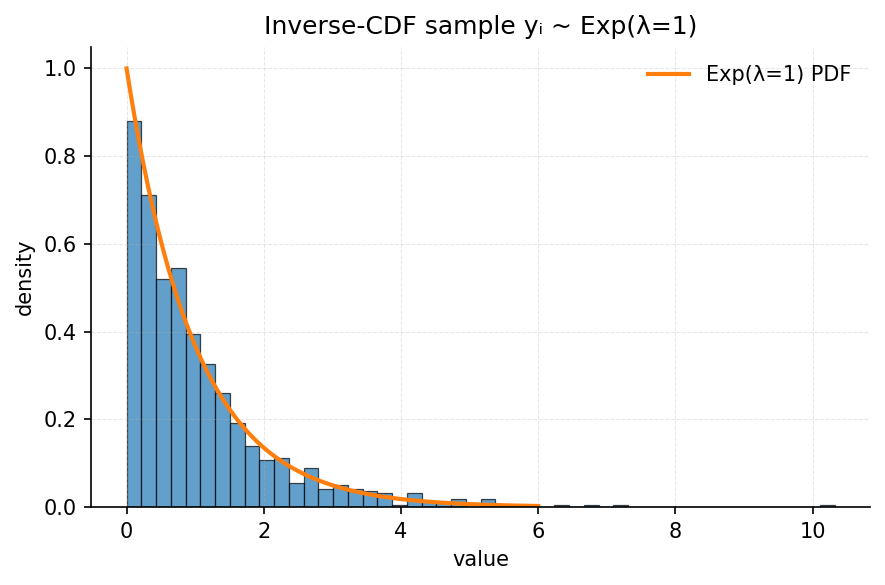
\includegraphics[width=0.5\linewidth]{q2b.png}
                \end{figure}
                
            \end{solution}
            
        \item Simulate 1000 random variables $z_1,\dots,z_{1000}$ with exponential distribution with parameter $\lambda=1$.

            \begin{solution}
    
\begin{lstlisting}[language=python]
import numpy as np
import matplotlib.pyplot as plt

SAMPLE_SIZE: int = 1000
RNG_SEED_2: int = 39  # Different seed to ensure different draws

rng2 = np.random.default_rng(RNG_SEED_2)

z = rng2.exponential(scale=1.0, size=SAMPLE_SIZE)

plot_exp_hist(z, title="Direct sample z_i ~ Exp(\lambda=1)")
\end{lstlisting}

                \begin{figure}[ht]
                    \centering
                    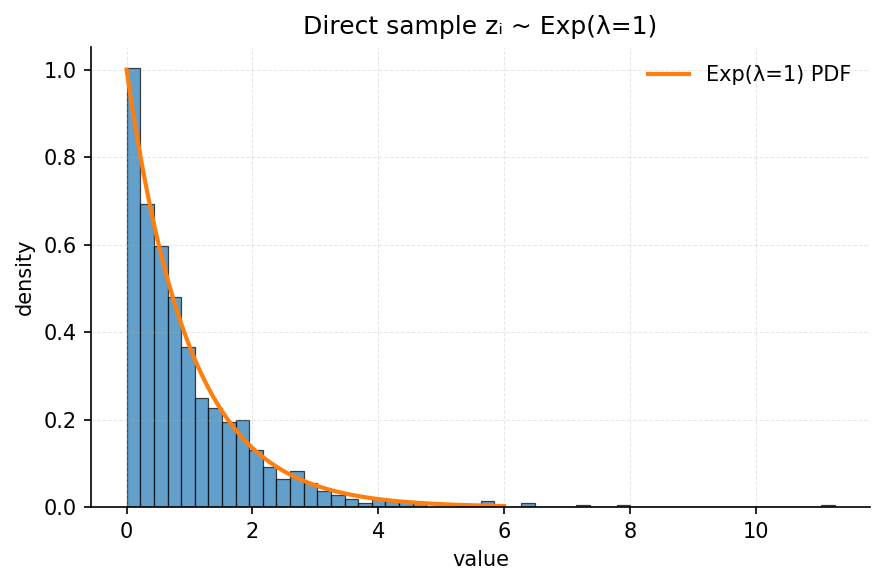
\includegraphics[width=0.5\linewidth]{q2c.png}
                \end{figure}
                
            \end{solution}
            
        \item Compare the histogram of the $y_i$ with the histogram of the $z_i$.

            \begin{solution}
    
\begin{lstlisting}[language=python]
y_f = y[np.isfinite(y)]
z_f = z[np.isfinite(z)]

# 1) Kolmogorov-Smirnov two-sample test
ks = stats.ks_2samp(y_f, z_f, alternative="two-sided", method="auto")

# 2) Cramer-von Mises two-sample test
cvm = stats.cramervonmises_2samp(y_f, z_f)

# 3) Wasserstein-1 distance
w1 = stats.wasserstein_distance(y_f, z_f)

print(f"KS test:                 D = {ks.statistic:.4f}, p = {ks.pvalue:.4g}")
print(f"Cramer-von Mises test:   T = {cvm.statistic:.4f}, p = {cvm.pvalue:.4g}")
print(f"Wasserstein-1 distance:  W-1 = {w1:.4f}")
\end{lstlisting}

                Across 1,000 draws, the two‐sample tests show no evidence that the samples differ: KS $D=0.047$ ($p=0.219$) and Cramer–von Mises $T=0.313$ ($p=0.124$) both fail to reject the null that $y_i$ (inverse-CDF) and $z_i$ (direct) come from the same distribution. The Wasserstein distance $W_1=0.071$ is small in the natural units of the variable (for $\mathrm{Exp}(1)$, $\sigma=1$), i.e., about 7\% of one standard deviation—well within Monte Carlo variability. 

                Overall, the results are consistent with both methods producing i.i.d. $\mathrm{Exp}(1)$ samples, confirming the correctness of the inverse-transform step.
            \end{solution}
            
    \end{enumerate}

\end{document}
